\begin{figure}[htbp]
  \begin{tabular}{cc}
    \begin{minipage}{0.5\hsize}
      \centering
      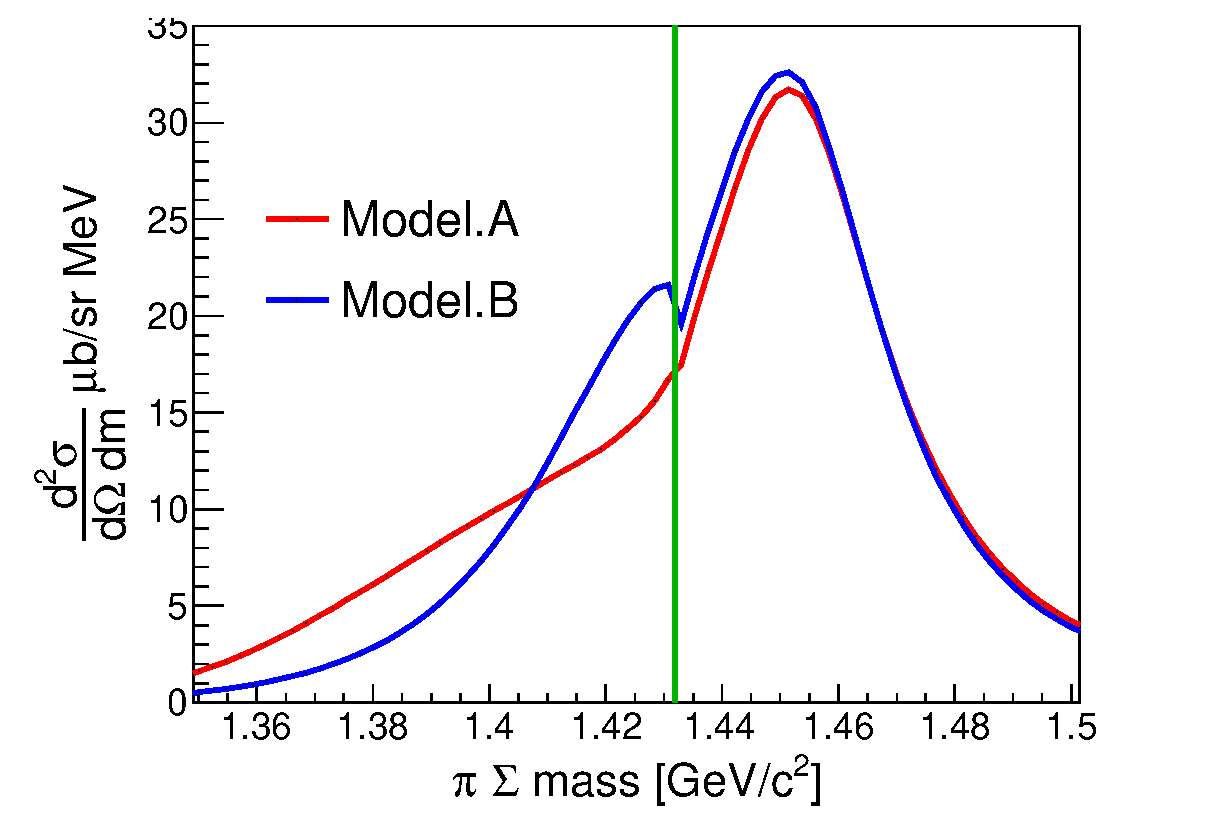
\includegraphics[width=6.0cm]{../pic/Dron/discussion/DCC_pimSp.eps}
    \end{minipage}
    
    \begin{minipage}{0.5\hsize}
      \centering
      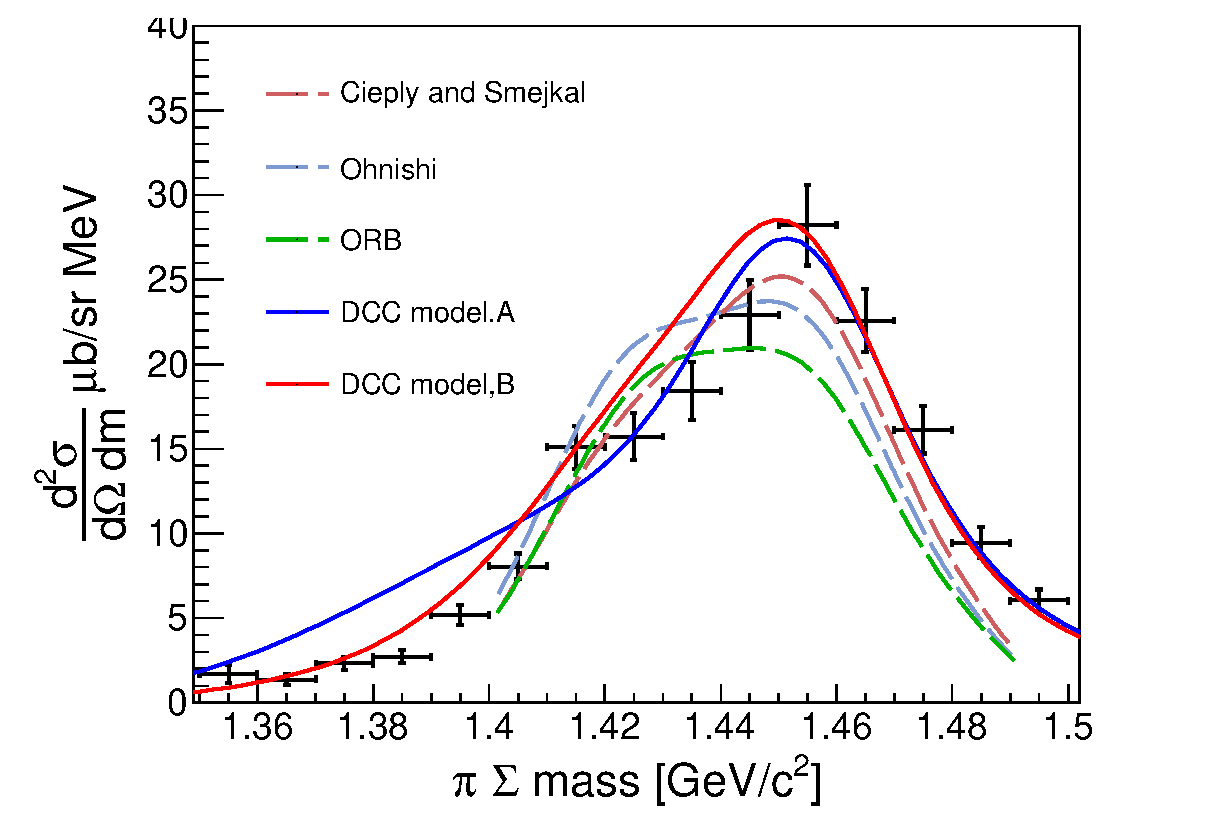
\includegraphics[width=6.0cm]{../pic/Dron/discussion/miyagawa_pimSp.eps}
    \end{minipage}
  \end{tabular}

  \begin{tabular}{cc}
    \begin{minipage}{0.5\hsize}
      \centering
      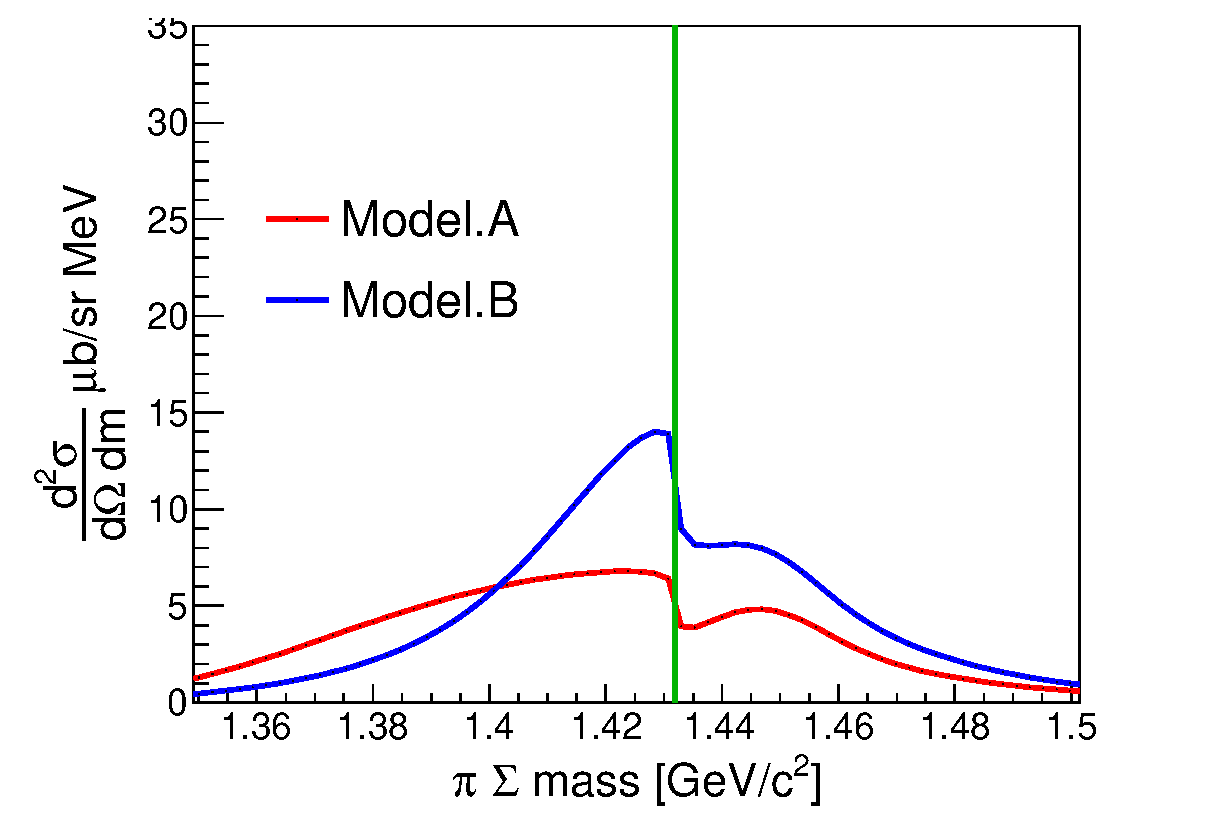
\includegraphics[width=6.0cm]{../pic/Dron/discussion/DCC_pipSm.eps}
    \end{minipage}
    
    \begin{minipage}{0.5\hsize}
      \centering
      \includegraphics[width=6.0cm]{../pic/Dron/discussion/miyagawa_pipSm.eps}
    \end{minipage}
  \end{tabular}

  \begin{tabular}{cc}
    \begin{minipage}{0.5\hsize}
      \centering
      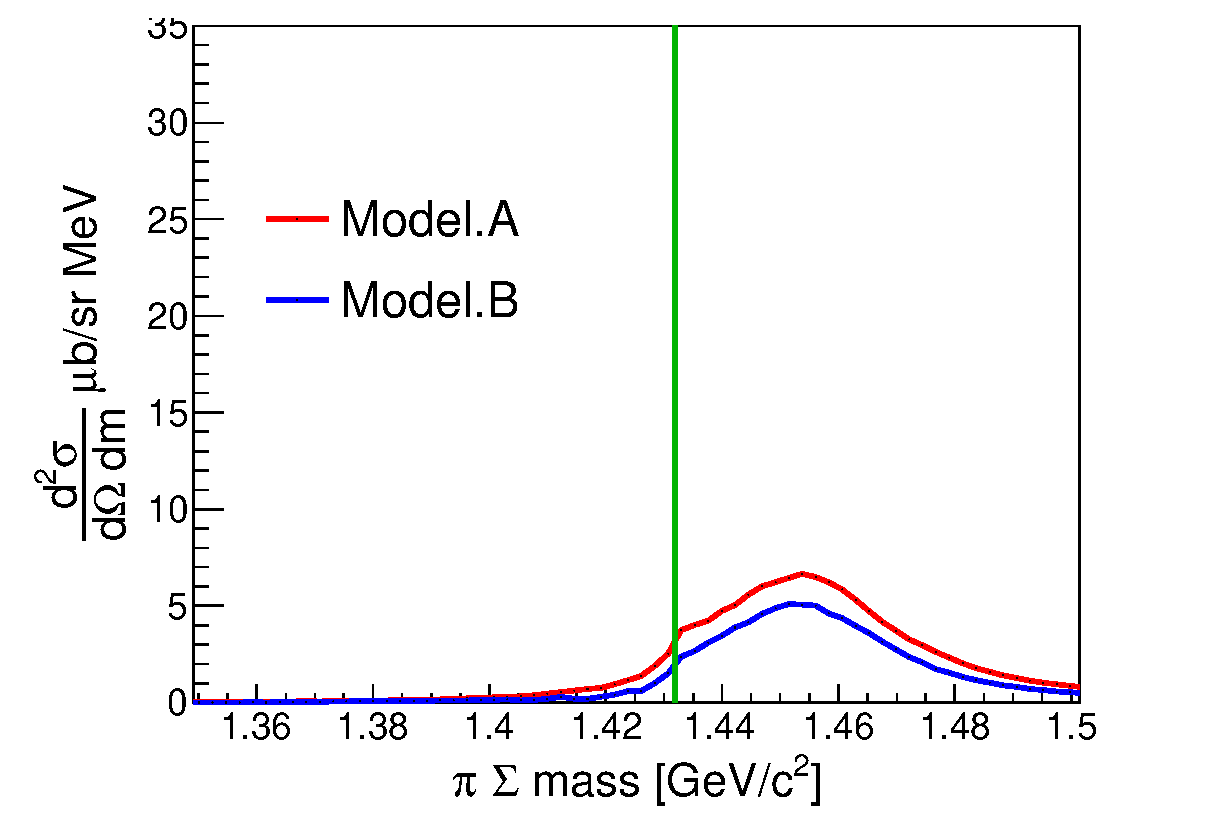
\includegraphics[width=6.0cm]{../pic/Dron/discussion/DCC_pimS0.eps}
    \end{minipage}
    
    \begin{minipage}{0.5\hsize}
      \centering
      \includegraphics[width=6.0cm]{../pic/Dron/discussion/miyagawa_pimS0.eps}
    \end{minipage}
  \end{tabular}
  
  \caption{
    This figure shows a comparison of our obtained spectra with predictions from theoretical calculations.
    The top, middle, and bottom figures represent $\pi^-\Sigma^+$, $\pi^+\Sigma^-$, and $\pi^-\Sigma^0$, respectively.
    The right figure shows the spectrum predicted by the DCC model, and the left figure shows the spectrum predicted by the calculation of Miyagawa et al.
    The spectra predicted by theoretical calculations are convoluted with our detector resolution.
  }
  \label{fig:comp_theoretical_calc}
\end{figure}


The previous section discussed the qualitative features of the obtained spectra.
In this section, we examine how well the reaction can be understood by comparing the data with theoretical calculations that take into account the kinematics of this experiment.

Two theoretical calculations are used for this purpose.
One is the \textit{hybrid} calculation by Miyagawa et al.\cite{Miyagawa}, which separates the reaction into
a first-step high-energy $K^-N \rightarrow \bar{K}N$ scattering and
a second-step low-energy $\bar{K}N\rightarrow \pi \Sigma$ scattering, which is the main focus.
In the second-step, three different scattering amplitudes obtained from various analyses of the $\Lambda(1405)$ are used.
This is to say, this method allows the second-step scattering amplitudes to be substituted with results from any $\Lambda(1405)$ analysis.
The other method is the DCC method, which treats these energy regions in a unified manner and uses continuous scattering amplitudes for both scatterings.
In this method, there are two sets of datasets, A and B, with the main uncertainty due to the lack of scattering data in the low energy region.

Figure \ref{fig:comp_theoretical_calc} shows a comparison between the experimental data and the predicted spectra from theoretical calculations.
The theoretical spectra are convolved with the detector resolution described in Appendix \ref{sec:detectr_reso}.
From top to bottom, the $\pi^+\Sigma^-$, $\pi^-\Sigma^+$, and $\pi^-\Sigma^0$ spectra are shown.
The right column shows the results from the DCC method \cite{DCC2},
and the left column shows those from the \textit{hybrid} calculation by Miyagawa et al.\cite{Miyagawa}.

The spectral shapes calculated by the two theoretical methods reproduce well the qualitative features discussed in the previous section.
Specifically, the $\pi^-\Sigma^0$ spectrum with an $I=1$ contribution exhibits a bump structure reflecting the first-step scattering,
while the $\pi^{\mp}\Sigma^{\pm}$ spectra, which include $I=0$, $I=1$, and their interference components,
show a clear structure below the $\bar{K}N$ threshold.
The difference observed between the $\pi^+\Sigma^-$ and $\pi^-\Sigma^+$ spectra,
which originates from the interference between the $I=0$ and $I=1$ components, is also reasonably well reproduced by the calculations.

However, the spectra predicted by the DCC method are well reproduced, both in shape and intensity.
In contrast, the \textit{hybrid} calculation reasonably reproduces the $\pi^+\Sigma^-$ spectrum in both shape and intensity,
but significantly overestimates the intensity of the $\pi^-\Sigma^+$ spectrum and underestimates that of the $\pi^-\Sigma^0$ spectrum.

This implies that a continuous treatment of the first- and second-step scattering is essential for understanding the present reaction.
That is to say, consistency with the higher-energy region is important for understanding $\bar{K}N$ scattering in the $\Lambda(1405)$ region.

The following discussion focuses on the spectra calculated by the DCC method.

%% In the previous section, we discussed the qualitative properties of the spectrum;
%% in this section,
%% we will examine our spectrum in more detail by comparing it with the kinematics-based theoretical calculations for this experiment.
%% These calculations assume that the reaction is a 2-step reaction described in Chapter 1,
%% which, as discussed in the previous section, is reasonable based on the $d(K^-, n)K^0 n$ spectrum.

%% Theoretical calculations of this experiment have been published by Miyagawa et al. \cite{Miyagawa}
%% and by Kamano et al. using the Dynamical Coupled Channel (DCC) method \cite{DCC2}.
%% The method of Miyagawa et al. employs the results of partial wave analysis for the first step $K^- N \rightarrow \bar{K}N$ scattering
%% and the results of various chiral analyses for the second step $\bar{K}N \rightarrow \pi \Sigma$ scattering,
%% i.e., these two scattering amplitudes are not continuously connected.
%% % Hybrid modelを使った場合
%% % The method of Miyagawa et al. employs the results of partial wave analysis for the first step, $K^- N \rightarrow \bar{K}N$ scattering,
%% % and various chiral analysis results for the second step, $\bar{K}N \rightarrow \pi \Sigma$ scattering, forming a so-called hybrid model.
%% % This approach means that the two scattering amplitudes are not continuously connected

%% On the other hand, the DCC method fits almost all available $K^- p \rightarrow$ meson-baryon scattering data over a wide mass range
%% to obtain the scattering amplitudes, and the scattering amplitudes of the first and second steps can be connected continuously.
%% The $\bar{K}N \rightarrow \pi \Sigma$ scattering amplitude used by Miyagawa et al. includes three variations:
%% a historical analysis by E. Oset, A. Ramos, and C. Bennhold \cite{ORB};
%% an analysis by Ohnishi et al. using the AGS equation \cite{Ohnishi};
%% and an analysis by A. Ciepl\'{y} and J. Smejkal utilizing SHIDDARTA data \cite{WT1}.
%% The two sets of parameters, known as Model A and Model B, are provided by the DCC method.
%% The pole parameters of the $\Lambda(1405)$, which has $I=0$ and is located below the $\bar{K}N$ threshold,
%% differ significantly due to the lack of low-momentum data
%% Figure \ref{fig:comp_theoritical_calc} shows our data alongside the theoretical calculations.
%% The spectra of $\pi^-\Sigma^+$, $\pi^+\Sigma^-$, and $\pi^-\Sigma^0$ are presented from the top panel downwards.
%% The left panels display the results obtained using the DCC method, while the right panels show the calculations by Miyagawa et al..

%% The spectral shapes of all theoretical calculations appear to reproduce the characteristics of all pi Sigma modes in the data we observed.
%% However, while the DCC method explains the strength for all $\pi \Sigma$ modes,
%% the Miyagawa et al. calculations are in good agreement for $\pi^- \Sigma^+$,
%% but greatly exceed the values of our observed data for $\pi^+ \Sigma^-$ and fall far short for $\pi^- \Sigma^0$.
%% The $\pi^- \Sigma^0$ spectrum has $I=0$, while the $\pi^{\mp} \Sigma^{\pm}$ spectrum exhibits both $I=0$ and $I=1$ effects.
%% Changes in one affect the other, making it challenging to achieve a comprehensive fit in Miyagawa's calculations.
%% This suggests the importance of establishing a continuous connection between the responses of the first step and the second step,
%% i.e., a consistent scattering amplitude in widly region.
